\pagestyle{empty}
\section{Entity Interaction\\{\small\tt J.~Mitchard}}
\label{entity_interactions}
As explained in section \ref{sys_overview_architecture}, the simulation has been implemented with a tile-viewer architecture. Whilst this allows for the the system to run more efficiently, it meant that a slightly more creative way of entities maintaining awareness had to be created. This section will cover the specifics of how tile and viewer processes interact, and how each entity interacts with them throughout the simulation.

\subsection{Tiles and Viewers}
\label{tiles_and_viewers}
When the map of tiles and viewers are created by \emph{environment.fsm}, they are each assigned a unique viewer along with the viewers of all of the neighbouring tile processes. This creates a grid as shown in section \ref{tile_viewer_diagram}. The purpose of these viewers is to allow entities to ask the viewer for their current tile what is around them, or, more specifically, what other entities are currently located on the same tile and in each of those surrounding it.

Each tile updates each of the viewers making up it's 'neighbourhood' of local tiles and viewers with new data regarding which entities are on it and where. Each tile reports to it's viewers from four sets of data held in it's state. These are:
\begin{description}
  \item[zombie\textunderscore map] - A map of each zombie currently on the tile with the zombies Process ID as the key.
  \item[human\textunderscore map] - A map of each human currently on the tile with the humans Process ID as the key.
  \item[item\textunderscore map] - A map of each item currently on the tile with the items Process ID as the key.
  \item[obs\textunderscore list] - A list of obstructed coordinates in the tile.
\end{description}

\subsection{Keeping the System Current}
Each time an entity moves, enters or leaves a tile, the tile in which the action has taken place will update it's associated neighbouring viewers with a new set of data relating to the type of entity that has been updated. For example, if a zombie moves from one position within the tile to another, the tile would only update the viewers with it's zombie data, rather than that of the items or humans as well.

The viewer holds similar information to the tiles, however instead of mapping each individual process as a key, it is mapped by tile with a list of entities as the values. This allows for a simple method of updating the viewer processes.

Because these data sets change so often and unpredictably, Erlang Maps are perfect for the job as when new data is inserted into the map with a pre existing key, the values are overwritten with the new set. This is considerably quicker than having to iterate through a list and changing it's value.

\subsection{Entities and Awareness}
\label{entities_awareness}
\label{viewer_intro}
In order for humans and zombies to have an awareness of their surroundings, it is necessary for them to ask the Viewer process for their current Tile for information; regarding nearby zombies, items, obstacles, and other humans. Because this information is constantly changing, it will have to do this at the start of each cycle of its state machine.

However, because each entity has a defined line of sight that is considerably less than the length and height of three tiles, which is what the viewer would provide information for, these lists will have to be filtered down to have this taken into consideration.

Firstly, each list is filtered to remove entities further than a defined distance away, the line of sight varies between humans and zombies. Secondly, the list uses the \emph{findline} function from the \emph{los.erl} module, which is introduced in section \ref{los}, to filter out entities in which line of sight is obstructed by obstacles. This will provide each entity with the information needed to make informed decisions of what to do next.

\subsection{Example of Process Communication}
This diagam shows an example snapshot of communication between a human, tile and viewer processes in which the human  requests information from the viewer, and then requests to move to a new position. The example assumes that the requested position was not obstructed.
\begin{figure}[h]
  \centering
  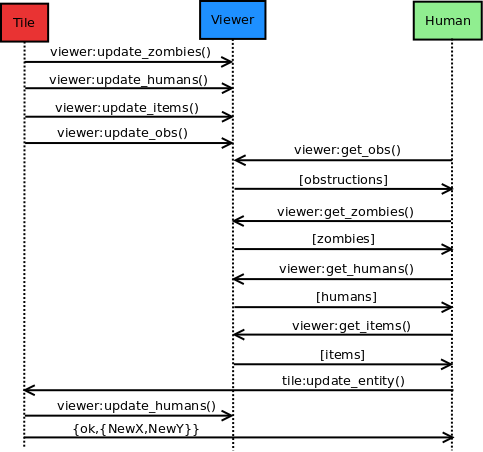
\includegraphics[width=0.6\textwidth]{img/tile-viewer-human-msgs.png}
  \caption{Human, Tile and Viewer Communication}
  \label{fig:tile_viewer_communication}
\end{figure}

\clearpage
\endinput
